\section{Theoretical Introduction}

\subsection{Social Homophily}

\subsection{Spearman's Coefficient}

Spearman's Rank Correlation Coefficient (also known as Spearman's rho) is a nonparametric measure of rank correlation which measures how well the relationship between two variables can be described using a monotonic function\cite{statistical_analysis}. Unlike Pearson's Correlation Coefficient, which measures lineal relationship between variables, Spearman's Coefficient uses the \emph{rank} of the variables in its calculations; therefore is measures its monotonicity.

For a sample of size \( n \) with scores \( X_i \) and \( Y_i \), the Spearman Coefficient \( r_s \) is defined as

\begin{equation}
r_s = \mathlarger{\rho}_{\rank(X) \rank(Y)} = \frac{\operatorname{cov}(\rank(x), \rank(y))}{\sigma_{\rank(X)} \sigma_{\rank(Y)}}
\label{spearman}
\end{equation}

Where \( \rho_{a,b} \) denotes the Pearson correlation between the variables \( a \) and \( b \). This value will be close to 1 when the variables are directly monotonic, close to -1 when they are inversely monotonic, and close to 0 when there is no tendency for either variable to increase or decrease when the other increases.

\subsection{Bayesian Inference}

This work uses a Bayesian approach to statistics instead of the usual Frequentist approach. In the Frequentist point of view, parameters are fixed and unknown: hypotheses are either true or false, and they cannot be described with a probability. In the Bayesian approach, anything unknown is described with a probability distribution since uncertainty must be described by probability.

The Bayesian approach connects the data \( x \) with a \emph{prior distribution} \( f \left( \theta \right) \) through the \emph{likelihood function} \( f \left( x \middle| \theta \right) \). Instead of estimating the value of \( \hat{\theta} \), the parameter that maximizes the likelihood, Bayesian inference is based on the evaluarion of the \emph{posterior distribution} \( f \left( \theta \middle| x \right) \).

By Bayes Theorem, we can infer the \emph{posterior distribution} using the other parameters.

\begin{equation}
f \left( \theta \middle| x \right) = \frac{f \left( x \middle| \theta \right) f \left( \theta \right)}{f \left( x \right)}
\label{bayes}
\end{equation}

\( f \left( x \right) \), the \emph{marginal likelihood}, is the probability of observing the data \( x \) averaged across the entire space, which acts as a normalizing constant so that the density integrates to 1.

\begin{equation}
f \left( x \right) = \int f \left( x \middle| \theta \right) f \left( \theta \right) d\theta
\label{marginal}
\end{equation}

\subsubsection{Beta Distribution}

In this context, the \emph{Beta distribution} is a family of Bayesian probability distributions which can be used to describe initial knowledge concerning probability of success of a single bi-variate distribution.

\begin{equation}
\Beta \left( x; \alpha, \beta \right) = \frac{1}{\Beta \left( \alpha, \beta \right)} x^{\alpha - 1} \cdot {\left( 1 - x \right)}^{\beta - 1}
\label{Beta}
\end{equation}

Where \( \alpha \) and \( \beta \) are parameters for the Beta distribution, and \( \Beta \) is the \emph{Beta function}, which is the normalizing constant of the distribution.

\begin{equation}
\Beta \left( \alpha, \beta \right) = \int^1_0 p^{\alpha - 1} {(1 - p)} ^{\beta - 1} dp = \frac{\Gamma (\alpha) \cdot \Gamma(\beta)}{\Gamma (\alpha + \beta)}
\label{Betaf}
\end{equation}

As we get more data from the sampling, the \emph{Beta distribution} turns more concenteated towards the actual \( \theta \) and its shapes resembles more a normal curve, as can be seen in \Cref{betagraph}. This represents the increased certainty which comes from the aquired knowledge of the problem.

\begin{figure}[H]
\begin{center}
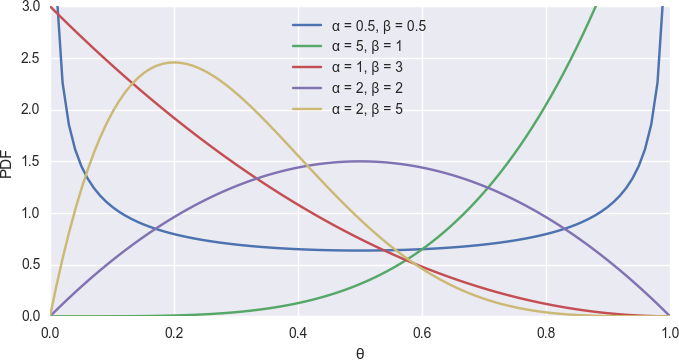
\includegraphics[width=\textwidth]{figures/beta.png}
\caption{Beta distribution with different parameters}
\end{center}
\label{betagraph}
\end{figure}
